\newcommand{\svcourse}{CST Part IA: Software Engineering and Security}
\newcommand{\svnumber}{1}
\newcommand{\svvenue}{Microsoft Teams}
\newcommand{\svdate}{2022-05-11}
\newcommand{\svtime}{15:00}
\newcommand{\svuploadkey}{CBd13xmL7PC1zqhNIoLdTiYUBnxZhzRAtJxv/ytRdM1r7qIfwMsxeVwM/pPcIo8l}

\newcommand{\svrname}{Dr Sam Ainsworth}
\newcommand{\jkfside}{oneside}
\newcommand{\jkfhanded}{yes}

\newcommand{\studentname}{Harry Langford}
\newcommand{\studentemail}{hjel2@cam.ac.uk}


\documentclass[10pt,\jkfside,a4paper]{article}

\usepackage{graphicx}
\usepackage{physics}
\usepackage{float}

% DO NOT add \usepackage commands here.  Place any custom commands
% into your SV work files.  Anything in the template directory is
% likely to be overwritten!

\usepackage{fancyhdr}

\usepackage{lastpage}       % ``n of m'' page numbering
\usepackage{lscape}         % Makes landscape easier

\usepackage{verbatim}       % Verbatim blocks
\usepackage{listings}       % Source code listings
\usepackage{graphicx}
\usepackage{float}
\usepackage{epsfig}         % Embed encapsulated postscript
\usepackage{array}          % Array environment
\usepackage{qrcode}         % QR codes
\usepackage{enumitem}       % Required by Tom Johnson's exam question header

\usepackage{hhline}         % Horizontal lines in tables
\usepackage{siunitx}        % Correct spacing of units
\usepackage{amsmath}        % American Mathematical Society
\usepackage{amssymb}        % Maths symbols
\usepackage{amsthm}         % Theorems

\usepackage{ifthen}         % Conditional processing in tex

\usepackage[top=3cm,
            bottom=3cm,
            inner=2cm,
            outer=5cm]{geometry}

% PDF metadata + URL formatting
\usepackage[
            pdfauthor={\studentname},
            pdftitle={\svcourse, SV \svnumber},
            pdfsubject={},
            pdfkeywords={9d2547b00aba40b58fa0378774f72ee6},
            pdfproducer={},
            pdfcreator={},
            hidelinks]{hyperref}

\renewcommand{\headrulewidth}{0.4pt}
\renewcommand{\footrulewidth}{0.4pt}
\fancyheadoffset[LO,LE,RO,RE]{0pt}
\fancyfootoffset[LO,LE,RO,RE]{0pt}
\pagestyle{fancy}
\fancyhead{}
\fancyhead[LO,RE]{{\bfseries \studentname}\\\studentemail}
\fancyhead[RO,LE]{{\bfseries \svcourse, SV~\svnumber}\\\svdate\ \svtime, \svvenue}
\fancyfoot{}
\fancyfoot[LO,RE]{For: \svrname}
\fancyfoot[RO,LE]{\today\hspace{1cm}\thepage\ / \pageref{LastPage}}
\fancyfoot[C]{\qrcode[height=0.8cm]{\svuploadkey}}
\setlength{\headheight}{22.55pt}


\ifthenelse{\equal{\jkfside}{oneside}}{

 \ifthenelse{\equal{\jkfhanded}{left}}{
  % 1. Left-handed marker, one-sided printing or e-marking, use oneside and...
  \evensidemargin=\oddsidemargin
  \oddsidemargin=73pt
  \setlength{\marginparwidth}{111pt}
  \setlength{\marginparsep}{-\marginparsep}
  \addtolength{\marginparsep}{-\textwidth}
  \addtolength{\marginparsep}{-\marginparwidth}
 }{
  % 2. Right-handed marker, one-sided printing or e-marking, use oneside.
  \setlength{\marginparwidth}{111pt}
 }

}{
 % 3. Alternating margins, two-sided printing, use twoside.
}


\setlength{\parindent}{0em}
\addtolength{\parskip}{1ex}

% Exam question headings, labels and sensible layout (courtesy of Tom Johnson)
\setlist{parsep=\parskip, listparindent=\parindent}
\newcommand{\examhead}[3]{\section{#1 Paper #2 Question #3}}
\newenvironment{examquestion}[3]{
\examhead{#1}{#2}{#3}\setlist[enumerate, 1]{label=(\alph*)}\setlist[enumerate, 2]{label=(\roman*)}
\marginpar{\href{https://www.cl.cam.ac.uk/teaching/exams/pastpapers/y#1p#2q#3.pdf}{\qrcode{https://www.cl.cam.ac.uk/teaching/exams/pastpapers/y#1p#2q#3.pdf}}}
\marginpar{\footnotesize \href{https://www.cl.cam.ac.uk/teaching/exams/pastpapers/y#1p#2q#3.pdf}{https://www.cl.cam.ac.uk/\\teaching/exams/pastpapers/\\y#1p#2q#3.pdf}}
}{}


\begin{document}

\section{Example Sheet 2}

As before, I assume the following imports before all code fragments:
\begin{lstlisting}[language=Python]
import random
import numpy as np
import pandas as pd
import scipy.stats as stats
import scipy.optimize as opt
from sklearn.linear_model import LinearRegression
\end{lstlisting}

\begin{enumerate}

\item Define a function \texttt{rxy()} that produces a random pair of values
$(X, Y)$ which, when shown in a scatter plot, produces a smiley face like
this. Also plot the marginal distributions of $X$ and $Y$.

\begin{lstlisting}[language=Python]
def circle(n):
	theta = 2 * np.random.random(n) * np.pi
	mu = np.column_stack([np.cos(theta), np.sin(theta)])
	return stats.norm.rvs(mu, 0.05)

def smile(n):
	theta = (np.random.random(n) - 1.5) * np.pi / 2
	mu = np.column_stack([np.cos(theta), np.sin(theta)])
	return 0.5 * stats.norm.rvs(mu, 0.05)

def left_eye(n):
	return stats.norm.rvs([-0.25, 0.25], 0.05, (n, 2))

def right_eye(n):
	return stats.norm.rvs(0.25, 0.05, (n, 2))

def face(n):
	p = [0.8, 0.15, 0.025, 0.025]
	return np.array([circle(n), smile(n), lefteye(n), righteye(n)])[
		np.random.choice([0,1,2,3], p=p, size=n), np.arange(n)]

\end{lstlisting}

\begin{figure}[H]
\centering
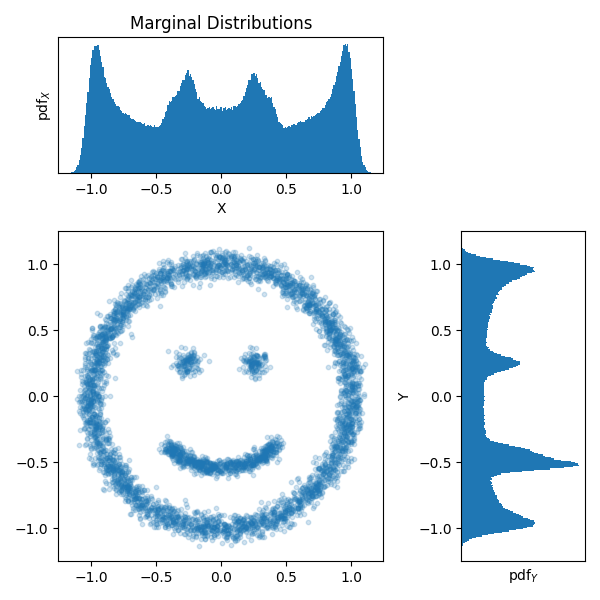
\includegraphics[width=0.6\textwidth]{./smiley_marginal_distribution}
\end{figure}

\item Consider this code for generating random variables $X$ and $Y$:

\begin{lstlisting}[language=Python]

x = np.random.uniform()
y = np.random.geometric(p=x)

\end{lstlisting}

Derive the marginal likelihood $\text{Pr}_Y(y)$ and the conditional
likelihood $\text{Pr}_X(x \ | \ Y = y)$.

The marginal likelihood $\text{Pr}_Y(y)$ is gained by integrating
$\text{Pr}_Y(y \ | \ X = x)\text{Pr}_X(x)$ over the valid range for $X$ --
in this case $[0, 1]$. We can do this using integration by parts.

\[
\begin{split}
\text{Pr}_Y(y)
&= \int^1_0 \text{Pr}_Y(y \ | \ X = x) \cdot \text{Pr}_X(x) \text{d}x \\
&= \int^1_0 (1 - x)^{y - 1}x \cdot 1 \text{d}x \\
&= \int^1_0 (1 - x)^{y - 1}x \text{d}x \\
&= \left[ - \frac{1}{y} x(1 - x)^y\right]^1_0 + \frac{1}{y}\int^1_0 (1 - x)
^2 \text{d}x \\
&= -\frac{1}{y(y + 1)}\left[ (1 - x)^{y + 1} \right]^1_0 \\
&= \frac{1}{y(y + 1)} \\
\end{split}
\]

The conditional likelihood $\text{Pr}_X(x \ | \ Y = y)$ can be derived using
Bayes rule:

\[
\begin{split}
\text{Pr}_X(x \ | \ Y = y)
&= \frac{\text{Pr}_X(x)\cdot\text{Pr}_Y(y \ | \ X = x)}{\text{Pr}_Y(y)} \\
&= \frac{1 \cdot (1 - x)^{y - 1}x}{\frac{1}{y(y + 1)}} \\
&= xy(y + 1)(1 - x)^{y-1} \\
\end{split}
\]

\iffalse

\item Sketch the cumulative distribution function and calculate the density
function for this continuous random variable:

\begin{lstlisting}[language=Python]
def rx():
	u = random.random()
	return u * (1 - u)
\end{lstlisting}

\[
\begin{split}
\mathbb{P}(rx < x)
&= \mathbb{P}(u(1 - u) < x) \\
&= \mathbb{P}\left(u < \frac{1}{2} - \sqrt{\frac{1}{4} - x}\right) +
\mathbb{P}\left(u > \frac{1}{2} + \sqrt{\frac{1}{4} - x}\right) \\
&= \frac{1}{2} - \sqrt{\frac{1}{4} - x} + 1 - \left( \frac{1}{2} +
\sqrt{\frac{1}{4} - x} \right) \\
&= \frac{1}{2} - \sqrt {\frac{1}{4} - x} + 1 - \frac{1}{2} - \sqrt
{\frac{1}{4} - x} \\
&= 1 - \sqrt {1 - 4x} \\
\end{split}
\]

Therefore the cumulative distribution function is:

\begin{figure}[H]
\centering
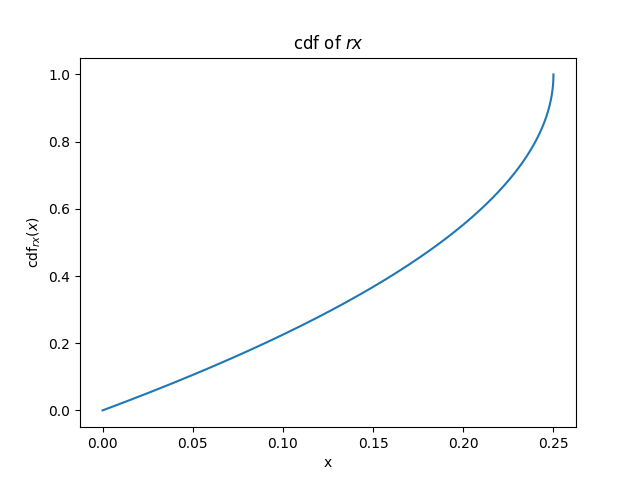
\includegraphics[width=0.5\textwidth]{./cdf_rx}
\end{figure}

We can obtain the pdf by differentiating the cdf.

\[
\begin{split}
\text{pdf}_{rx}
&= \dv{\text{cdf}_{rx}}{x} \\
&= \frac{2}{\sqrt{1 - 4x}} \\
\end{split}
\]

\begin{figure}[H]
\centering
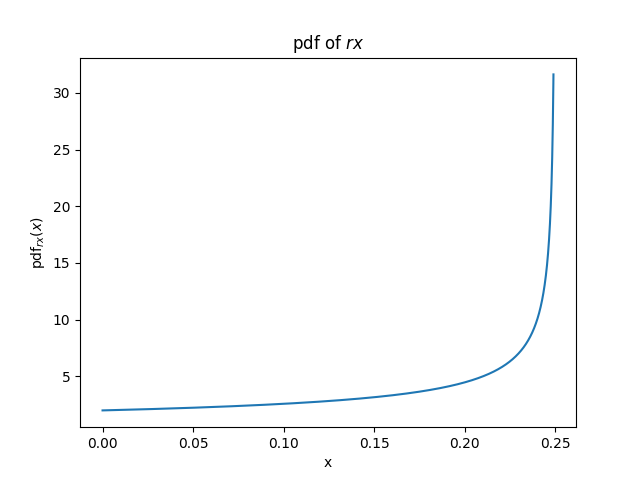
\includegraphics[width=0.5\textwidth]{./pdf_rx}
\end{figure}

\fi

\item I sample $x_1, \dots, x_n$ from Uniform$[0, \theta]$. The parameter
$\theta$ is unknown and I shall use $\Theta \sim \text{Pareto}(b_0,
\alpha_0)$ as my prior, where $b_0 > 0$ and $\alpha_0 > 1$ are known. This
has the cumulative distribution function:
\[
\mathbb{P}(\Theta \leq \theta) =
\begin{cases}
1 - \left( \frac{b_0}{\theta} \right)^{\alpha_0} & \text{if} \ \theta \geq
b_0 \\
0 & \text{if} \ \theta < b_0 \\
\end{cases}
\]

\begin{enumerate}[label=(\alph*)]

\item Calculate the prior likelihood for $\Theta$.

The prior likelihood for $\theta$ is given by $\pdv{\mathbb{P}}{\theta}$.
This is equal to:

\[
\begin{split}
\text{pdf}_{\Theta}(\theta) &=
\begin{cases}
\frac{\alpha_0 b_0^{\alpha_0}}{\theta^{\alpha_0 - 1}} & \ \text{if} \ \theta
\geq b_0 \\
0 & \text{otherwise}
\end{cases} \\
&= \frac{\alpha_0 b_0^{\alpha_0}}{\theta^{\alpha_0 - 1}}1_{\theta \geq b_0} \\
\end{split}
\]

\item Show that the posterior distribution of $(\Theta | x_1, \dots, x_n)$
is Pareto and find its parameters.

We can find the posterior distribution using Bayes rule.

\[
\begin{split}
\Pr(\theta | x_1, \dots, x_n)
&= \frac{\Pr\left(\theta\right) \cdot \Pr\left(x_1, \dots, x_n | \theta\right)
}{\Pr(x_1, \dots x_n)} \\
&= \frac{\frac{\alpha_0 b_0^{\alpha_0}}{\theta^{\alpha_0 - 1}}1_{\theta \geq
b_0} \frac{1}{\theta^n}1_{\theta \geq \text{max}_i x_i}}{\Pr(x_1, \dots x_n)} \\
&= \frac{\alpha_0 b_0^{\alpha_0}}{\Pr(x_1, \dots x_n)
}\frac{1}{\theta^{\alpha_0 + n- 1}}1_{\theta
\geq b_0}1_{\theta \geq \text{max}_i x_i}\\
&= \kappa \frac{1}{\theta^{\alpha_0 + n- 1}}1_{\theta
\geq \text{max}\left(b_0, \text{max}_i x_i\right)} \text{ for some constant }
\kappa \\
&= \frac{\kappa}{\left( \alpha_0 + n \right)(\text{max}\left(b_0, \text{max}_i x_i\right))^{\alpha_0 + n}}
\text{Pareto}(\text{max}\left(b_0, \text{max}_i x_i\right), \alpha_0 + n) \\
\end{split}
\]

Since the whole function integrates to 1 over $(0, \infty)$ and $\text{Pareto}
(\text{max}\left(b_0, \text{max}_i x_i\right), \alpha_0 + n)$ also integrates to 1 over $(0, \infty)$, we can
conclude that $\kappa = \left(\alpha_0 + n \right)(\text{max}\left(b_0, \text{max}_i x_i\right))^{\alpha_0 + n}$
and therefore the distribution itself is $\text{Pareto}(\text{max}\left(b_0, \text{max}_i x_i\right), \alpha_0 + n)$.

Therefore the posterior distribution for $\theta$ is $\text{Pareto}
(\text{max}\left(b_0, \text{max}_i x_i\right), \alpha_0 + n)$..

\item Find a 95\% posterior confidence interval for $\Theta$.

We can find the inverse cumulative distribution function for pareto and use
this to find $\theta$ such that $\mathbb{P}(\Theta < \theta) = 0.95$.

\[
\begin{split}
p &= 1 - \left(\frac{\text{max}\left(b_0, \text{max}_i x_i\right)}{\theta}\right)^{\alpha_0 + n} \\
1 - p &= \left(\frac{\text{max}\left(b_0, \text{max}_i x_i\right)}{\theta}\right)^{\alpha_0 + n} \\
\frac{1}{\sqrt[\alpha_0 + n]{\frac{1}{1-p}}} &= \frac{\text{max}\left(b_0, \text{max}_i x_i\right)}{\theta} \\
\theta &= \sqrt[\alpha_0 + n]{\frac{1}{1-p}}\text{ max}\left(b_0,
\text{max}_i x_i\right) \\
\end{split}
\]

Setting $p = 0.95$ gives $\text{cdf}_\theta\left(\sqrt[\alpha_0 +
n]{20}\text{ max}\left(b_0, \text{max}_i x_i\right)\right) = 0.95$

Therefore a 95\% confidence interval for $\Theta$ is $[\text{max}\left(b_0, \text{max}_i x_i\right),
\sqrt[\alpha_0 + n]{20} \text{ max}\left(b_0, \text{max}_i x_i\right)]$

\item Find a different 95\% posterior confidence interval. Which is better?
Why?

Alternatively we could find values such that
$\mathbb{P}(\Theta < \theta) = 0.025$ and
$\mathbb{P}(\Theta < \theta) = 0.975$. This would give a 95\% confidence interval

Plugging these values into the inverse cdf calculated earlier gives
$\text{cdf}_\theta\left(\sqrt[\alpha_0 + n]{\frac{40}{39}}\text{ max}\left
(b_0, \text{max}_i x_i\right)\right) = 0.025$
and $\text{cdf}_\theta\left(\sqrt[\alpha_0 + n]{40}\text{ max}\left(b_0,
\text{max}_i x_i\right)\right) = 0.975$

Therefore another 95\% confidence interval for $\Theta$ is
$\left[\sqrt[\alpha_0 + n]{\frac{40}{39}}\text{ max}\left(b_0, \text{max}_i
x_i\right), \sqrt[\alpha_0 +
n]{40}\text{ max}\left(b_0, \text{max}_i x_i\right)\right]$.

Neither of these 95\% confidence intervals is ``better'' than the other.
However, I would argue that the second is more useful than the first in
many cases.

\end{enumerate}

\item I have a collection of numbers $x_1, \dots, x_n$ which I take to be
independent samples from the $\mathcal{N}(\mu, \sigma_0^2)$ distribution.
Here $\sigma_0$ is known, and $\mu$ is unknown. Using the prior distribution
$M \sim \mathcal{N}(\mu_0, \rho_0^2)$ for $\mu$, show that the posterior
distribution is:

\[
\text{Pr}_M(\mu | x_1, \dots, x_n) = \kappa e^{-\frac{(\mu - c)^2}{2\tau^2}}
\]

where $\kappa$ is a normalising constant and where you should find formulae
for $c$ and $\tau$ in terms of $\sigma_0$, $\mu_0$, $\rho_0$ and the $x_i$.
Hence deduce that the posterior distribution is $\mathcal{N}(c, \tau^2)$.

Using Bayes rule:

\[
\begin{split}
\text{Pr}_M(\mu | x_1, \dots, x_n)
&= \frac{\text{Pr}_M\left(\mu)\cdot \text{Pr}_X(x_1, \dots,
x_n | \mu\right)}{\text{Pr}_X\left(x_1, \dots, x_n\right)} \\
&= \frac{\frac{1}{\sqrt{2\pi}\rho_0}e^{-\frac{\left( \mu - \mu_0 \right)^2}
{2\rho_0^2}}\prod^n_{i=1}\frac{1}{\sqrt{2\pi}\sigma_0}e^{-\frac{(x_i - \mu)
^2}{2\sigma_0^2}}}{\Pr\left(x_1, \dots, x_n\right)} \\
&= \kappa_0 e^{-\left( \frac{\left( \mu - \mu_0 \right)^2}{2\rho_0^2} +
\frac{\sum^n_{i=1}\left( \mu - x_i \right)^2}{2\sigma_0^2}\right)} \text{
for some constant }\kappa_0 \\
&= \kappa_0 e^{-\frac{\sigma_0^2\mu^2 -
2\sigma_0^2\mu_0\mu + n\rho_0^2\mu^2 - 2\rho_0^2\sum^n_{i=1}x_i}{2\sigma_0^2\rho_0^2} +
\kappa_1} \text{ for some constants } \kappa_0, \kappa_1 \\
&= \kappa_0 \ln \kappa_1 e^{-\frac{\left(\sigma_0^2 + n\rho_0^2\right)\mu^2 -
2\left( \sigma_0^2\mu_0 + \rho_0^2\sum^n_{i=1}x_i \right)
\mu}{2\sigma_0^2\rho_0^2}} \text{ for some constants } \kappa_0, \kappa_1 \\
&= \kappa_2 e^{-\frac{\mu^2 - 2\frac{\sigma_0^2\mu_0 +
\rho_0^2\sum^n_{i=1}x_i}{\sigma_0^2 +
n\rho_0^2}\mu}{2\frac{\sigma_0^2\rho_0^2}{\sigma_0^2 + n\rho_0^2}}}
\text{ for some constant } \kappa_2 \\
&= \kappa_2 e^{-\frac{\left( \mu - \frac{\sigma_0^2\mu_0 +
\rho_0^2\sum^n_{i=1}x_i}{\sigma_0^2 + n\rho_0^2} \right)
^2}{2\frac{\sigma_0^2\rho_0^2}{\sigma_0^2 + n\rho_0^2}} +
\frac{\left( \frac{\sigma_0^2\mu_0 +
\rho_0^2\sum^n_{i=1}x_i}{\sigma_0^2 + n\rho_0^2} \right)
^2}{2\frac{\sigma_0^2\rho_0^2}{\sigma_0^2 + n\rho_0^2}}}
\text{ for some constant } \kappa_2 \\
&= \kappa_3 e^{-\frac{\left( \mu - \frac{\sigma_0^2\mu_0 +
\rho_0^2\sum^n_{i=1}x_i}{\sigma_0^2 + n\rho_0^2} \right)
^2}{2\frac{\sigma_0^2\rho_0^2}{\sigma_0^2 + n\rho_0^2}}}
\text{ for some constant } \kappa_3 \\
\end{split}
\]

This is of the form:
\[
\text{Pr}_M(\mu | x_1, \dots, x_n) = \kappa e^{-\frac{(\mu - c)^2}{2\tau^2}}
\]

With
\begin{align*}
c &= \frac{\sigma_0^2\mu_0 +
\rho_0^2\sum^n_{i=1}x_i}{\sigma_0^2 + n\rho_0^2} & \tau &=
\frac{\sigma_0\rho_0}{\sqrt{\sigma_0^2 + n\rho_0^2}}
\end{align*}

These values pass sanity checks: for $n=0$ the posterior distribution is the
prior distribution $\mathcal{N}(\mu_0, \rho_0^2)$ and as $n\rightarrow \infty$,
the distribution approaches $\mathcal{N}\left( \frac{\sum^n_{i=1}x_i}{n},
\frac{\sigma^2_0}{n} \right)$ -- the distribution of the mean of the $x_i$.

\item I repeatedly attempt a task and each time I attempt it I succeed with
probability $\theta$ and fail with probability $1 - \theta$. The parameter
$\theta$ is unknown, so I model it as a random variable $\Theta$. Ever the
optimist, my prior for $\Theta$ is heavily biased in favour of large values
for $\theta$:

\[
\text{Pr}_{\Theta}\left( \theta \right) = \varepsilon1_{\theta \leq
\frac{1}{2}} + (2 - \varepsilon)1_{\theta \geq \frac{1}{2}}
\]

for some known small value $\varepsilon > 0$; this implies
$\mathbb{P}\left( \Theta \leq \frac{1}{2} \right) = \frac{\varepsilon}{2}$.

But I experience an unbroken run of $n$ failures. How big does $n$ need to
be for me to concede there's a 50\% posterior probability that
$\Theta \leq \frac{1}{2}$? How big would it need to be if $\varepsilon = 0$?

For the purposes of this question I will assume the \textit{only
observations we have} are this unbroken run of $n$ failures. Without this
assumption, the question is unanswerable.

The probability of $\Theta < \frac{1}{2}$ given a sequence of $n$ failures
is given by:
\[
\varepsilon\int^{\frac{1}{2}}_0 \left( 1 - \theta \right)^n \dd{\theta}
\]

The probability of $\theta \geq \frac{1}{2}$ given a sequence of $n$
failures is given by:
\[
\left( 2 - \varepsilon \right)\int^1_{\frac{1}{2}} \left( 1 - \theta \right)^n
\dd{\theta}
\]

If the probability of $\theta < \frac{1}{2}$ is $50\%$ then these two
probabilities must be equal to each other: they are the only two cases
and the probability of all cases sums to 1 so the other probability must be
100\% - 50\% = 50\%. We can therefore equate them and solve.

\[
\begin{split}
\varepsilon\int^{\frac{1}{2}}_0 \left( 1 - \theta \right)^n \dd{\theta}
&= \left( 2 - \varepsilon \right)\int^1_{\frac{1}{2}} \left( 1 - \theta
\right)^n \dd{\theta} \\
\frac{\varepsilon}{n+1}\left[-\left( 1 - \theta \right)
^{n+1}\right]^{\frac{1}{2}}_0
&= \frac{2 - \varepsilon}{n+1}\left[-\left( 1 - \theta \right)
^{n+1}\right]^1_{\frac{1}{2}} \\
\varepsilon\left( 1 - \frac{1}{2}^{n+1} \right) &= \left( 2 - \varepsilon
\right)\frac{1}{2}^{n+1} \\
\varepsilon &= \frac{1}{2}^{n} \\
n &= -\lg \varepsilon \\
\end{split}
\]

So to concede that there is a 50\% posterior probability that $\Theta \leq
\frac{1}{2}$, we need to observe an unbroken run of $-\lg \varepsilon$
failures.

If $\varepsilon = 0$, then we could never be convinced our probability of
failure was $\leq \frac{1}{2}$. If the probability of an event in the prior
distribution is zero, then the probability of that event in the posterior
distribution is always zero.

\item I have a collection of numbers

\[
[4.3, 2.8, 3.9, 4.1, 9, 4.5, 3.3]
\]

which look like they mostly come from a Gaussian distribution, but with the
occasional outlier. Model the data as

\[
X \sim
\begin{cases}
\mathcal{N}\left(\mu, 0.5^2\right) & \text{ with probability } 99\% \\
\text{Cauchy} & \text{ with probability } 1\%
\end{cases}
\]

Use a $\mathcal{N}(0, 5^2)$ prior distribution for $\mu$. Give pseudocode to
plot the posterior distribution.

\begin{lstlisting}[language=Python]
n = 5000000
observed = [4.3, 2.8, 3.9, 4.1, 9, 4.5, 3.3]
data = np.full((n, len(observed)), observed)
p = np.random.random(size=data.shape)
logprob = np.empty_like(data)
logprob[p >= 0.99] = stats.cauchy.logpdf(data[p >= 0.99])
mus = stats.norm.rvs(0, 5, n)
logprob[p < 0.99] = stats.norm.logpdf(np.column_stack([mus]), data, 0.5)[p < 0.99]
logprob = np.sum(logprob, axis=1)
prob = np.exp(logprob - np.max(logprob))
"""
bins is so large because we're plotting a lot of data outside the
graph. We can resolve this by either cropping data or zooming into
the part we care about by generating points with scipy.stats.truncnorm
"""
plt.hist(mus, weights=prob, bins=500, density=True)
plt.show()
\end{lstlisting}

\begin{figure}[H]
\centering
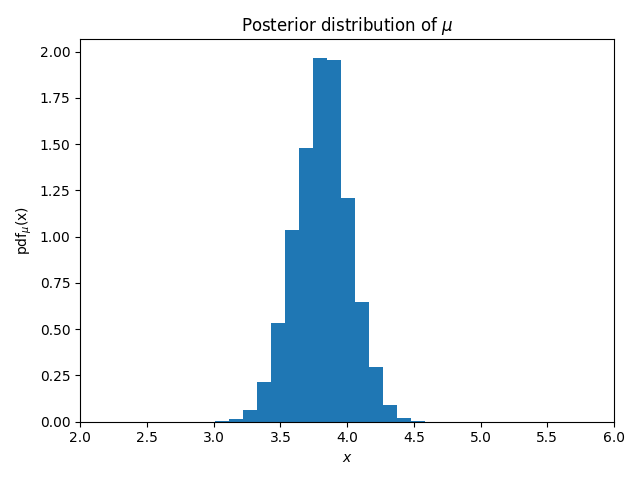
\includegraphics[width=0.5\textwidth]{./posterior_distribution_mu_cauchy_and_normal}
\end{figure}

\item In lecture notes section 2.6 we investigated a dataset of police
stop-and-search actions. Let the outcome for record $i$ be $y_i \in \{0,
1\}$, where 1 denotes that the police found something and 0 denotes that
they found nothing. Consider the probability model $Y_i\sim B(1,
\beta_{\text{eth}})$ where eth$_i$ is the recorded ethnicity for the
individual involved in record $i$, ans where the parameters
$\beta_{\text{As}}$, $\beta_{\text{Blk}}$, $\beta_{\text{Mix}}$,
$\beta_{\text{Oth}}$, $\beta_{\text{Wh}}$ are unknown. As a prior
distribution, suppose that the five $\beta$ parameters are all independent
$\beta\left(\frac{1}{2}, \frac{1}{2}\right)$ random variables.

\begin{enumerate}[label=(\alph*)]

\item Write down the joint prior density for ($\beta_{\text{As}}$, $\beta_{\text{Blk}}$, $\beta_{\text{Mix}}$,
$\beta_{\text{Oth}}$, $\beta_{\text{Wh}}$).

Since the $\beta$ are independent, the joint probability density function is
the product of the individual probability density functions. Therefore,
using the probability density function for the $\beta\left( \frac{1}{2},
\frac{1}{2}\right)$ distribution; the joint probability density function is
given by:

\[
\begin{split}
\text{Pr}(\beta_{\text{As}},\dots, \beta_{\text{Wh}})
&= \prod_{\text{eth}} \frac{\beta_{\text{eth}}^{\frac{1}{2} - 1}\left( 1 -
\beta_{\text{eth}}
\right)^{\frac{1}{2} - 1}}{\left( \frac{\Gamma\left(\frac{1}{2}\right)\Gamma\left( \frac{1}{2} \right)}{\Gamma\left( \frac{1}{2} + \frac{1}{2} \right)
}\right)} \\
&= \prod_{\text{eth}} \frac{\beta_{\text{eth}}^{-\frac{1}{2}}\left( 1 -
\beta_{\text{eth}}
\right)^{-\frac{1}{2}}}{\left( \frac{\Gamma\left(\frac{1}{2}\right)^2}{\Gamma\left( 1 \right)
}\right)} \\
&= \prod_{\text{eth}} \frac{\beta_{\text{eth}}^{-\frac{1}{2}}\left( 1 -
\beta_{\text{eth}}
\right)^{-\frac{1}{2}}}{\left( \frac{\Gamma\left(\frac{1}{2}\right)
^2}{1}\right)} \\
&= \prod_{\text{eth}}\frac{1}{\Gamma\left( \frac{1}{2} \right)^2\sqrt 
{\beta_\text{eth}(1 - \beta_\text{eth})}}
\end{split}
\]

\item Find the joint posterior distribution of ($\beta_{\text{As}}$, $\beta_{\text{Blk}}$, $\beta_{\text{Mix}}$,
$\beta_{\text{Oth}}$, $\beta_{\text{Wh}}$) given the $y$ data.

Using Bayes rule:

\[
\begin{split}
\Pr(\beta_{\text{As}}, \dots, \beta_{\text{Wh}}| Y) &=
\frac{\Pr(\beta_{\text{As}}, \dots, \beta_{\text{Wh}})\cdot
\Pr(Y | \beta_{\text{As}}, \dots, \beta_{\text{Wh}})}{\Pr(Y)} \\
&= \kappa_1 \prod_{\text{eth}}\frac{1}{\Gamma\left( \frac{1}{2} \right)^2\sqrt
{\beta_\text{eth}(1 - \beta_\text{eth})
}}\beta_{\text{eth}}^{\sum^{n}_{i=1}y_i 1_{\text{eth}_i=\text{eth}}}
\left( 1 - \beta_{\text{eth}} \right)^{\sum^{n}_{i=1}(1 - y_i)1_{\text{eth}_i=\text{eth}} } \\
&= \kappa_2 \prod_{\text{eth}}\beta_{\text{eth}}^{\left(\sum^{n}_{i=1}y_i
1_{\text{eth}_i=\text{eth}}\right) - \frac{1}{2}}\left( 1 -
\beta_{\text{eth}} \right)^{\left(\sum^{n}_{i=1}(1 - y_i)1_{\text{eth}_i=\text{eth}}\right) - \frac{1}{2}} \\
&= \prod_{\text{eth}}\beta\left(\frac{1}{2} + \sum^{n}_{i=1}y_i
1_{\text{eth}_i=\text{eth}}, \frac{1}{2} + \sum^{n}_{i=1}(1 - y_i)
1_{\text{eth}_i=\text{eth}}\right) \\
\end{split}
\]

Where the $\beta$ on the line above denotes the probability density
function of a $\beta$ distribution with the given parameters.

\end{enumerate}

\item I am prototyping a diagnostic test for a disease. In healthy patients,
the test result is $\mathcal{N}(0, 2.1^2)$. In sick patients it is
$\mathcal{N}(\mu, 3.2^2)$, but I have not yet established a firm value for
$\mu$. In order to estimate $\mu$, I trialled the test on 30 patients whom
I know to be sick and the mean test result was 10.3. I subsequently apply
the test to a new patient and get the answer 8.8. I wish to know whether
this new patient is healthy or sick.

\begin{enumerate}[label=(\alph*)]

\item In this question there are two unknown quantities: $\mu$ and $h \in
\{\text{healthy}, \text{sick}\}$ the status of the new patient. Model the
former as a random variable $M$ with prior distribution $\mathcal{N}(5, 3^2)$
and the latter as a random variable $H$ with prior distribution

\[
\text{Pr}_H(h) = 0.99 \times 1_{h=\text{healthy}} + 0.01\times 1_{h=\text{sick}}
\]

Write down the joint prior likelihood for $(M, H)$.

Since $M$ and $H$ are independent, the joint prior likelihood is the product
of their individual likelihoods.

\[
\text{Pr}(M, H) = \left( 0.99 \cdot 1_{h=\text{healthy}} + 0.01
\cdot 1_{h=\text{sick}} \right) \cdot
\frac{1}{\sqrt{2\pi}\cdot3}e^{-\frac{\left(
\mu - 5 \right)^2}{2\cdot 3^2}}
\]

\item In this question the data consists of 31 values, test results $x_1,
\dots, x_{30}$ from the known sick patients and test result $y$ from the new
patient. Write down the data likelihood $\Pr(x_1, \dots, x_{30}, y| \mu, h)$.

\[
\begin{split}
\Pr(x_1, \dots, x_{30}, y| \mu, h)
&= \Pr(y \ | \ \mu, h) \cdot \Pr(x_1, \dots, x_30 \ | \ \mu, h) \\
&= \left(\frac{1_{h=\text{healthy}}}{\sqrt{2\pi}2.1} e^{-
\frac{y^2}{2 \cdot 2.1^2}} + \frac{1_{h=\text{sick}}}{\sqrt
 {2\pi}3.2} e^{-\frac{\left( \mu - y \right)^2}{2\cdot 3.2^2}} \right)\prod^{30}_{i=1} \frac{1}{\sqrt{2\pi}\cdot
3.2}e^{-\frac{\left( \mu - x_i \right)^2}{2 \cdot 3.2^2}} \\
&= \frac{1}{\sqrt {2\pi}^{31}\cdot3.2^{30}}\left( \frac{
1_{h=\text{healthy}}}{2.1}e^{-\frac{y^2}{{2 \cdot 2.1^2}}} + \frac{
1_{h=\text{sick}}}{3.2} e^{-\frac{\left( \mu - y \right)^2}{{2 \cdot 3.2^2}}}
\right) e^{-\frac{\sum^{30}_{i=1}\left( \mu - x_i \right)^2}{{2 \cdot 3.2^2}}} \\
\end{split}
\]

\item Find the posterior density of $(M, H)$. Leave your answer as an
unnormalised density function. It should simplify to be a function of
$\bar{x}$ and $y$ where $\bar{x}$ is the mean test result for the known sick
patients.

\[
\begin{split}
\Pr(\mu, h | x_1, \dots, x_{30}, y)
&= \frac{\Pr_{M, H}(\mu, h) \Pr\left(x_1, \dots, x_{30}, y| \mu, h\right)}{
\Pr\left( x_1, \dots, x_{30}, y \right) } \\
&= \kappa_0 \text{Pr}_{M, H}(\mu, h) \Pr \left(x_1, \dots, x_{30}, y| \mu,
h\right) \\
&= \kappa_1 e^{-\frac{\left( \mu - 5 \right)^2}{2\cdot 3^2}}
\left( \frac{ 0.99\cdot 1_{h=\text{healthy}}}{2.1}e^{-\frac{y^2}{{2 \cdot 2.1^2}}} +
\frac{0.01 \cdot 1_{h=\text{sick}}}{3.2} e^{-\frac{\left( \mu - y \right)^2}{{2 \cdot 3.2^2}}}
\right) e^{-\frac{\sum^{30}_{i=1}\left( \mu - x_i \right)^2}{2 \cdot 3.2^2}} \\
&= \kappa_2 e^{-\frac{\left( \mu - 5 \right)^2}{2\cdot 3^2}}
\left( \frac{ 0.99\cdot 1_{h=\text{healthy}}}{2.1}e^{-\frac{y^2}{{2 \cdot 2.1^2}}} +
\frac{0.01 \cdot 1_{h=\text{sick}}}{3.2} e^{-\frac{\left( \mu - y \right)^2}{{2 \cdot 3.2^2}}}
\right) e^{-\frac{30\mu^2 - 2\mu\sum^{30}_{i=1}x_i}{2 \cdot 3.2^2}} \\
&= \kappa_3 e^{-\frac{\left( \mu - 5 \right)^2}{2\cdot 3^2}}
\left( \frac{ 0.99\cdot 1_{h=\text{healthy}}}{2.1}e^{-\frac{y^2}{{2 \cdot 2.1^2}}} +
\frac{0.01 \cdot 1_{h=\text{sick}}}{3.2} e^{-\frac{\left( \mu - y \right)^2}{{2 \cdot 3.2^2}}}
\right) e^{-\frac{\left(\mu - \frac{\mu\sum^{30}_{i=1}x_i}{30}\right)^2}{2
\cdot \left(\frac{3.2}{\sqrt{30}}\right)^2}} \\
&= \kappa_3 e^{-\frac{\left( \mu - 5 \right)^2}{2\cdot 3^2}}
\left( \frac{ 0.99\cdot 1_{h=\text{healthy}}}{2.1}e^{-\frac{y^2}{{2 \cdot 2.1^2}}} +
\frac{0.01 \cdot 1_{h=\text{sick}}}{3.2} e^{-\frac{\left( \mu - y \right)^2}{{2 \cdot 3.2^2}}}
\right) e^{-\frac{\left(\mu - \bar{x}\right)^2}{2
\cdot \left(\frac{3.2}{\sqrt{30}}\right)^2}} \\
\end{split}
\]

\item Give pseudocode to compute the posterior distribution of $H$, i.e.\
compute $\mathbb{P}\left( H=h|\text{data} \right)$ for both
$h=\text{healthy}$ and $h=\text{sick}$.

\begin{lstlisting}[language=Python]
xs = [...]
y = ...
n = 100000

def logprob(xs, y, mus, h):
	broadcast_xs = np.full((n, len(xs)), xs)
	broadcast_mu = np.full((len(xs), n), mus).transpose()
	logpdfs = stats.norm.logpdf(broadcast_xs, broadcast_mu, 3.2)
	logpr_x = np.sum(logpdfs, axis=1)
	if h == 'healthy':
		logpr_y = stats.norm.logpdf(y, 0, 2.1)
	else:
		logpr_y = stats.norm.logpdf(y, mu, 3.2)
	return logpr_x + logpr_y

mus = stats.norm.rvs(3, 5, n)

healthy_logpr = logprob(xs, y, mus, 'healthy')
healthy_logpr = np.exp(healthy_logpr - np.max(healthy_logpr))

sick_logpr = logprob(xs, y, mus, 'sick')
sick_logpr = np.exp(sick_logpr - np.max(sick_logpr))

fig, (ax1, ax2) = plt.subplots(2)

ax1.hist(mu, weights=healthy_logpr, density=True, bins=k)
ax2.hist(mu, weights=healthy_logpr, density=True, bins=k)

\end{lstlisting}

\end{enumerate}

\item In the lecture notes on linear modelling, we proposed a linear model
for a temperature increase:

\[
\mathbf{temp} \approx \alpha + \beta_1\sin(2\pi \mathbf{t}) + \beta_2 \cos
(2\pi \mathbf{t}) + \gamma(\mathbf{t} = 2000)
\]

Suggest a probability model for $\mathbf{temp}$. Suggest Bayesian prior
distributions for the unknown parameters $\alpha$, $\beta_1$, $\beta_2$ and
$\gamma$. Give pseudocode to find a 95\% confidence interval for $\gamma$.

I propose that the residuals are normally distributed around the
prediction made by the linear model mean 0 and standard deviation $\sigma$.
Therefore the model can be rewritten as

\[
\mathbf{temp} \sim \alpha + \beta_1\sin(2\pi \mathbf{t}) + \beta_2 \cos
(2\pi \mathbf{t}) + \gamma(\mathbf{t} = 2000) + \mathcal{N}(0, \sigma^2)
\]

I suggest the following prior distributions for $\alpha$, $\beta_1$,
$\beta_2$ and $\gamma$:

\begin{align*}
\alpha &\sim \mathcal{N}(10, 1) \\
\beta_1 &\sim \mathcal{N}(-1, 0.5) \\
\beta_2 &\sim \mathcal{N}(-6, 0.5) \\
\gamma &\sim \mathcal{N}(0, 0.1) \\
\end{align*}

\begin{lstlisting}[language=Python]
n = 1000000
features = np.array([
		np.ones_like(climate.t),
		np.sin(2 * np.pi * climate.t),
		np.cos(2 * np.pi * climate.t),
		climate.t - 2000
		])

coefs = np.array([
		stats.norm.rvs(10, 1, n),
		stats.norm.rvs(-1, 0.5, n),
		stats.norm.rvs(-6, 0.5, n),
		stats.norm.rvs(0, 0.1, n)
		])

br_features = np.full((n, 4, climate.t.size), features)

br_coefs = np.full((climate.t.size, 4, n), coefs)

predictions = np.sum(br_features.transpose() * br_coefs, axis=1)
residuals = predictions - np.full((n, df.t.size), df.temp).transpose()
logprob = stats.norm.logpdf(residuals, 0, np.std(residuals, axis=0))
logprob = np.sum(logprob, axis=0)
prob = np.exp(logprob - np.max(logprob))
gammas = coefs[:, 3]
order = np.argsort(gammas)
gammas = gammas[order]
prob = prob[order] / np.sum(prob)
print(prob[np.cumsum(prob) > 0.025][0], prob[np.cumsum(prob) < 0.975][-1])
\end{lstlisting}

The output is 0.012644294207450358, 0.03886258682519564.

\end{enumerate}

\section{Supplementary question sheet 2}

\begin{enumerate}

\setcounter{enumi}{9}

\iffalse

\item 

\begin{enumerate}[label=(\alph*)]

\item For the random variables $X \sim \mathcal{U}[-1, 1]$ and
$Y \sim \mathcal{N}\left( X^2, 0.1^2 \right)$, compute the conditional
distribution of $\left(X \ | \ Y \in \left[ 0.5, 0.7 \right]\right)$.

\begin{lstlisting}[language=Python]
n = 5000000
xs = 2 * (np.random.random(size=n) - 0.5)
ys = stats.norm.rvs(xs ** 2, 0.1)
plt.hist(xs[(0.5 <= ys) & (ys <= 0.7)], bins=250, density=True)
\end{lstlisting}

\begin{figure}[H]
\centering
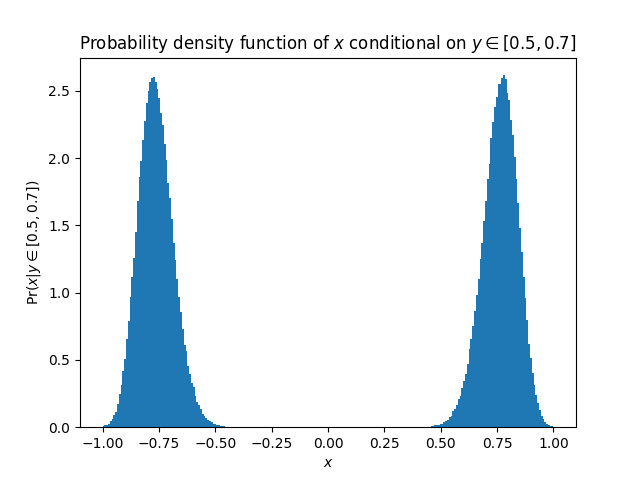
\includegraphics[width=0.5\textwidth]{./conditional_x_on_y_in_05_07}
\end{figure}

\end{enumerate}

\item

\begin{enumerate}[label=(\alph*)]

\item Let $T$ be the maximum of $m$ independent $\mathcal{U}[0, 1]$ random
variables. Show that $\mathbb{P}(T \leq t) = t^m$. Find the density function
$\text{Pr}_T(t)$.

Let $T_i$ be the largest of $i \geq 1$ random variables distributed by
$\mathcal{U}[0, 1]$. I will prove by induction that $\mathbb{P}(T_i \leq t) =
t^i$ which proves that $\mathbb{P}(T \leq t) = t^m$.

For $i=1$:
\[
\mathbb{P}(T_1 \leq t) = \mathbb{P}(\mathcal{U}[0, 1] \leq t) = t
\]

Assume that the theorem is true for $i = k$. I will then prove it is true for
$i = k + 1$:
\[
\mathbb{P}(T_{k+1} \leq t) = \mathbb{P}(\mathcal{U}[0, 1] \leq t) \mathbb{P}
(T_{k} \leq t)= t\cdot t^k = t^{k+1}
\]

Since the induction is true for $i = 1$ and if it is true for $i=k$ then it
must also be true for $i=k+1$; by induction it must therefore be true for
all $i\geq 1$. Therefore it is true for $i=m$ and so
$\mathbb{P}(T \leq t) = t^m$ as required.

Since we have worked out the cumulative distribution function $\mathbb{P}(T
\leq t)$, we can differentiate this to work out the probability
density function $\text{Pr}_T(t)$.

\[
\begin{split}
\text{Pr}_T(t) &= \dd{\mathbb{P}(T \leq t)}{t} \\
&= m \cdot t^{m - 1} \\
\end{split}
\]

\item A common task in data processing is counting the number of unique
items in a collection. When the collection is too large to hold in memory,
we may wish to use fast approximation methods, such as the following: Given
a collection of items $a_1, a_2, \dots$ compute the hash of each item
$x_1 = h\left(a_1\right), x_2 = h\left( a_2 \right), \dots$ then compute
$t = \text{max}_i \ x_i$.

If the hash function is well designed, then each $x_i$ can be treated as if
it were sampled from $\mathcal{U}[0, 1]$, and unequal items will yield
independent samples.

The more unique items there are, the larger we expect $t$ to be. Given an
observed value $t$, find the maximum likelihood estimator for the number of
unique items.

From the previous section, we have the probability density function for $T$.
To find the maximum likelihood estimator, we must differentiate this with
respect to $m$ and find the maximum.

\[
\begin{split}
\text{Pr}_T(t) &= m \cdot t^{m-1} \\
\pdv{\text{Pr}_T(t)}{m} &= m\cdot \ln t \cdot t^{m-1} + t^{m-1} \\
0 &= t^{m-1}\left( m\cdot \ln t + 1 \right) \\
0 &= \hat{m}\cdot \ln t + 1 \\
\hat{m} &= -\frac{1}{\ln t} \\
\hat{m} &= \log_{\frac{1}{e}} t \\
\end{split}
\]

\end{enumerate}

\item A point lightsource at coordinates $(0, 1)$ sends out a ray of light
at an angle $\Theta$ chosen uniformly in $[-\frac{\pi}{2}, \frac{\pi}{2}]$.
Let $X$ be the point where the ray intersects the horizontal line through
the origin. What is the density of $X$?

\[
\begin{split}
X &\sim \tan\Theta \\
\text{Pr}(X \leq x) &= \text{Pr}\left( \tan \Theta \leq x \right) \\
&= \text{Pr}\left( \Theta \leq \arctan x \right) \\
&= \frac{\pi + 2\arctan x}{2\pi} \\
\end{split}
\]

We can therefore distribute this to find the probability density function:

\[
\text{pdf}_X = \pdv{\frac{\pi + 2\arctan x}{2\pi}}{x} = \frac{1}{\pi(1 + x^2)}
\]

\fi

\item Consider this code for generating random variables $X \rightarrow Y
\rightarrow Z$.

\begin{lstlisting}[language=Python]
x = np.random.uniform()
y = np.random.binomual(n=1, p=x)
z = np.random.normal(loc=y, scale=epsilon)
\end{lstlisting}

Show that:
\[
\text{Pr}_Y\left( 1 | X = x, Z = z \right) = \frac{x}{x + (1 - x)e^{\frac{1-2z}{2\varepsilon^2}}}
\]

\[
\begin{split}
\text{Pr}_Y\left( 1 | X = x, Z = z \right)
&= \frac{\Pr_X(x)\Pr_Y(1 | x), \Pr_Z(Z | X, Y)}{\Pr_X(x)\Pr_Z(z | x)} \\
&= \frac{1 \cdot x \cdot \frac{1}{\sqrt{2\pi}\varepsilon} e^{-\frac{\left( z
- 1 \right)^2}{2\varepsilon^2}} }{1\cdot\left(\frac{x}{\sqrt{2\pi}\varepsilon}
e^{-\frac{\left( z - 1 \right)^2}{2\varepsilon^2}} + \frac{
(1 - x)}{\sqrt{2\pi}\varepsilon}e^{-\frac{z^2}{2\varepsilon^2}}\right)} \\
&= \frac{x\cdot e^{-\frac{\left( z - 1 \right)^2} {2\varepsilon^2}}}{x \cdot
 e^{-\frac{\left( z - 1 \right)^2}{2\varepsilon^2}} + (1 - x) \cdot
 e^{-\frac{z^2}{2\varepsilon^2}}} \\
&= \frac{x}{x + (1 - x) \cdot e^{\frac{(z - 1)^2 - z^2 }{2\varepsilon^2}}} \\
&= \frac{x}{x + (1 - x) \cdot e^{\frac{1 - 2z}{2\varepsilon^2}}} \\
\end{split}
\]


How does $\text{Pr}_Y\left( 1 | X = x, Z = z \right)$ depend on $x$ and $z$
when $\varepsilon \approx 0$? What if $\varepsilon$ is very large?

If $\varepsilon \approx 0$ then $\text{Pr}_Y\left( 1 | X = x, Z = z \right)
\approx e^{\frac{2z - 1}{2\varepsilon^2}}$. This assigns a very high
probability if $z > \frac{1}{2}$ and a very low probability if $z <
\frac{1}{2}$.

If $\varepsilon$ is very large then $\text{Pr}_Y\left( 1 | X = x, Z = z
\right) \approx x$ -- as the standard deviation of $z$ is so high that $z$
tells us very little.

\item Suppose we're given a function $f(x) \geq 0$ and we want to evaluate

\[
\int^b_{x=a} f(x) \dd{x}
\]

Here's an approximation method: (i) draw a box that contains $f(x)$ over the
range $x \in \left[ a, b \right] $, (ii) scatter points uniformly at random
in this box, (iii) return $A \times p$ where $A$ is the area of the box and
$p$ is the fraction of points that are under the curve. Explain why this is
a special case of Monte Carlo integration.

Consider taking a sample $(x, y)$ from inside a box $A$. The probability
that $y < f(x)$ for some function $f$ is equal to the proportion of the box
which is less than $f$. This is the definition of the integral of $f$
(potentially clipped) over $[a, b]$. Therefore $P(y < f(x)) =
\frac{\int^b_a f(x)\text{d}x}{A}$. Consider now a binomial random variable
$Z$ which takes $n$ such samples. By definition, $Z$ therefore has the
distribution $B(n, P(y < f(x))) = B\left(n, \frac{\int^b_a f(x)
\text{d}x}{A}\right)$.

By the expectation of binomial random variables:
\[
\begin{split}
\mathbb{E}\left( Z \right) &= nP(y < f(x)) \\
\end{split}
\]

By splitting $Z$ up into $n$ individual bernoulli trials $(x_i, y_i)$, we can
rewrite $Z$ as:
\[
Z = \sum^n_{i=1} 1_{y_i < f(x_i)}
\]

We can now combine these equations:
\[
\begin{split}
nP(y < f(x)) &= \mathbb{E}\left(\sum^n_{i=1} 1_{y_i < f(x_i)}\right) \\
nP(y < f(x)) &\approx \sum^n_{i=1} 1_{y_i < f(x_i)} \\
P(y < f(x)) &\approx \frac{1}{n}\sum^n_{i=1} 1_{y_i < f(x_i)} \\
\mathbb{E}\left(P(y < f(x))\right) &\approx \frac{1}{n}\sum^n_{i=1} 1_{y_i < f
(x_i)
} \\
\end{split}
\]

This is in the form of a Monte Carlo approximation; where we estimate the
probability $P(y < f(x))$ by drawing samples from a distribution which is 1
with probability $P(y < f(x))$.

Notice that $\frac{1}{n}\sum^n_{i=1} 1_{y_i < f(x_i)}$ is the fraction of
points under the curve -- $p$ and that by definition, $P(y < f(x)) = \frac{\int^b_a f(x)
\text{d}x}{A}$. Next, substitute these into the above formula:

\[
\begin{split}
\mathbb{E}\left(\frac{\int^b_a f(x)\text{d}x}{A}\right) &\approx p \\
\frac{\int^b_a f(x)\text{d}x}{A} &\approx p \\
\int^b_a f(x)\text{d}x &\approx A \times p \\
\end{split}
\]

This proves that the proposed approximation technique is valid.

\item I have a biased coin, with unknown probability of heads $\theta$. I
toss it $n$ times with outcomes $x_1, x_2, \dots, x_n$ where $x_i = 1$
indicates heads and $x_i = 0$ indicates tails. My prior belief is $\Theta
\sim \mathcal{U}[0, 1]$. Here are two approaches to applying Bayes's rule:
\begin{itemize}

\item \textit{One-shot Bayes}. Use Bayes's rule to compute the posterior of
$\Theta$, given data $(x_1, \dots, x_n)$, using prior $\Theta \sim
\mathcal{U}[0, 1]$ and assuming that coin tosses are independent.

\item \textit{Sequential Bayes}. Use Bayes's rule to compute the posterior
of $\Theta$ given data $x_1$ using the uniform prior; let the posterior
density be $p_1(\theta)$. Apply Bayes's rule again to compute the posterior
of $\Theta$ given data $x_2$, but this time using $p_1(\theta)$ as the
prior; let the posterior density be $p_2(\theta)$. Continue applying
Bayes's rule in this way until we have found $p_n(\theta)$.

\end{itemize}

State the posterior distribution found by one-shot Bayes. prove by induction
on $n$ that sequential Bayes gives the same answer.

The posterior distribution for $\theta$ found by one-shot Bayes is:
\[
\Theta \sim \beta\left( 1 + \sum^n_{i=1}x_i, 1 + n - \sum^n_{i=1}x_i \right)
\]

I will prove by induction that the posterior distribution found by
Sequential Bayes is the same:

For $n = 0$:

\[
\begin{split}
\text{Pr}_\Theta(\theta \ | \ )
&= \frac{\text{Pr}_\Theta(\theta)\Pr(1 \ | \ \theta)}{\Pr(1)} \\
&= \Pr_{\Theta} \\
&= 1 \\
&= \theta^0(1 - \theta)^0 \\
&\sim \beta\left(1 + \sum^{0}_{i=1}x_i, 1 + 0 - \sum^{0}_{i=1}x_i  \right) \\
\end{split}
\]

Therefore the result holds for $n = 0$.

Assume next that it holds for $n = k$ and calculate the posterior
probability for $n = k = 1$:

\[
\begin{split}
\text{Pr}_\Theta(\theta \ | \ x_1, \dots, x_{k+1})
&= \frac{\text{Pr}_\Theta(\theta \ | \ x_1, \dots, x_k)\Pr(x_{k+1} \ | \
\theta, x_1, \dots, x_k)}{\text{Pr}(x_{k+1})} \\
&= \kappa \cdot \theta^{\sum^k_{i=1}x_i}(1 - \theta)^{n - \sum^k_{i=1}x_i}
\cdot \theta^{x_{k+1}}(1 - \theta)^{1 - x_{k+1}} \\
&= \theta^{\sum^{k+1}_{i=1}x_i}(1 - \theta)^{n - \sum^{k+1}_{i=1}x_i} \\
&\sim \beta\left(1 + \sum^{k+1}_{i=1}x_i, 1 + n - \sum^{k+1}_{i=1}x_i\right) \\
\end{split}
\]

Therefore if the result holds for $n = k$, it must also hold for $n = k + 1$.
Since it holds for $n = 0$, we can conclude that for all $n \in \mathbb{N}$:

\[
\Pr(\Theta \ | \ x_1, \dots, x_n) \sim \beta\left(1 + \sum^n_{i=1}x_i, 1 + n -
\sum^n_{i=1}x_i\right)
\]

For the general case I will prove that the posterior probability for
$\text{Pr}(\theta_0, \dots, \theta_m \ | \ x_1, \dots x_n)$ obtained via
sequential bayes is the same as the result obtained using one-shot Bayes.

For $n = 0$, the result from Sequential Bayes bayes is equal to:

\[
\begin{split}
\text{Pr}(\theta_1, \dots, \theta_m \ | \ 1)
&= \frac{\text{Pr}(\theta_1, \dots, \theta_m)\text{Pr}(1 \ | \ \theta_1,
\dots, \theta_m)}{\text{Pr}(1)} \\
&= \text{Pr}(\theta_1, \dots, \theta_m) \\
\end{split}
\]

This is clearly the same as the result from one-shot Bayes.

Assume that for $n = k$, the result from Sequential Bayes is the same as the
result from One-Shot Bayes:

\[
\begin{split}
\text{Pr}(\theta_1, \dots, \theta_m \ | \ x_1, \dots x_{k+1})
&= \frac{\text{Pr}(\theta_1, \dots, \theta_m \ | \ x_1, \dots, x_k)
\text{Pr}(x_{k+1} \ | \ \theta_1, \dots, \theta_m, x_1, \dots, x_k)}{\text{Pr}
(x_{k+1})} \\
&= \frac{\text{Pr}(\theta_1, \dots, \theta_m \ | \ x_1, \dots x_{k+1})\text{Pr}
(x_{k+1} \ | \ \theta_1, \dots, \theta_m)}{\text{Pr}(x_{k+1})} \\
&= \frac{\frac{\text{Pr}(\theta_1, \dots, \theta_m)\text{Pr}(x_1, \dots, x_k
 \ | \ \theta_1, \dots, \theta_m)}{\text{Pr}(x_1, \dots, x_k)}\text{Pr}
(x_{k+1} \ | \ \theta_1, \dots, \theta_m)}{\text{Pr}(x_{k+1})} \\
&= \frac{\text{Pr}(\theta_1, \dots, \theta_m)\text{Pr}(x_1, \dots, x_{k+1}
 \ | \ \theta_1, \dots, \theta_m)}{\text{Pr}(x_1, \dots, x_{k+1})} \\
\end{split}
\]

This is the posterior distribution obtained by One-Shot Bayes. Therefore if
the posterior distribution obtained from Sequential Bayes with $k$
independent observations is equal to the posterior distribution obtained
from One-Shot Bayes with $k$ independent observations; then the posterior
distribution obtained from Sequential Bayes with $k + 1$ independent
observations is the same as the posterior distribution obtained from
One-Shot Bayes with $k + 1$ independent observations. Since the posterior
distributions obtained with zero observations were the same, we can conclude
by mathematical induction that for all $n \in \mathbb{N}$; the posterior
distributions obtained from One-Shot Bayes and Sequential Bayes are the same.

\item In the setting of question 7, I wish to measure the amount of police
bias. Given a 5-tuple of parameters $\beta = (\beta_{\text{As}},
\beta_{\text{Blk}}, \beta_{\text{Mix}}, \beta_{\text{Oth}},
\beta_{\text{Wh}})$, I define the overall bias score to be

\[
d(\beta) = \max_{e, e'}\left|\beta_e - \beta_{e'}\right|
\]

If $d(\beta)$ is large, then there is some pair of ethnicities with very
unequal treatment. As a Bayesian, I view $\beta$ as a random variable taking
values in $[0, 1]^5$, therefore $d(\beta)$ is a random variable also. To
investigate its distribution, I sample $\beta$ from the posterior
distribution that I found in question 7, I compute $d(\beta)$, and plot a
histogram. The output from the left is bizarre. To help me understand what's
going on, I plot histograms of each of the individual $\beta_e$
coefficients, shown here on the right.

Explain the results.

The beta distribution is U-shaped only when both parameters $\alpha$ and
$\beta$ are strictly less than 1. If there are any measurements for a given
ethnicity then one of the the parameters become strictly greater than 1: the
parameters are $\frac{1}{2} + \sum^n_{i=1}y_{i}1_{\text{eth}_i=\text{eth}}$
and $\frac{1}{2} + \sum^n_{i=1}(1 - y_i)1_{\text{eth}_i=\text{eth}}$.

Since the distribution for mixed is U-shaped, we can conclude that there are
no records of any people of mixed ethnicity being stop-and-searched in the
police dataset. This has skewed the posterior distribution of $d(\beta)$.

All ethnicities except for Mixed have data. Other has the least data, while
Black, White and Asian having a sufficient data for the
distribution to be moderately low.

\item Consider the outlier model from question 6. How likely is it that the
datapoint with value 9 is an outlier.

I will consider an ``outlier'' to be a datapoint generated according to the
Cauchy distribution.

Let $Z$ be $1_{X \sim \text{Cauchy}}$. Therefore the probability that the
datapoint with value 9 is an outlier is $\Pr(Z=1 \ | \ X=9)$. We can write this as
a probability model using Bayes rule for continuous random variables.

\[
\begin{split}
\Pr(Z=1 \ | \ X=9) &= \frac{\Pr(Z=1, X=9)}{\Pr(X=9)} \\
			 &= \frac{\Pr(Z=1, X=9)}{\Pr(Z=1, X=9) + \Pr(Z=, X=9)} \\
\end{split}
\]

The functions on both side are well behaved and therefore we can calculate
this explicitly. $\Pr(Z=1, X=9)$ is the probability density function of a
Cauchy distribution evaluated at value 9. Using the probability density
function for a Cauchy distribution:

\[
\begin{split}
\Pr(Z=1, X=x) &= \Pr(Z=1)\Pr(X=x \ | \ Z=1) \\
\Pr(Z=1, X=x) &= 0.01\cdot\frac{1}{\pi(1 + x^2)} \\
\end{split}
\]

The probability density function for $\Pr(Z=0, X=x)$ can be found by
integrating the product of the prior distribution $\Pr(\mu)$ and the
distribution $\Pr(X \ | \ Z=0)$ between $-\infty$ and $\infty$.

\[
\begin{split}
\Pr(Z=0, M=\mu, X=x)
&= \Pr(Z=0)\Pr(M=\mu \ | \ Z=0)\Pr(X=x \ | \ Z=0, M=\mu) \\
&= 0.99 \cdot \frac{1}{\sqrt{2\pi} \cdot 5^2}e^{-\frac{\mu^2}{2\cdot 5}} \cdot
\frac{1}{\sqrt{2\pi}\cdot 0.5} e^{ -\frac{(x - \mu)^2}{2\cdot 0.5^2} } \\
\end{split}
\]

We can therefore integrate this with respect to $\mu$ to work out
$\Pr(Z=0, X=x)$.

\[
\begin{split}
\Pr(Z=0, X=x)
&= \int^\infty_{-\infty} 0.99 \cdot \frac{1}{\sqrt{2\pi} \cdot
5}e^{-\frac{\mu^2}{2\cdot 5^2}} \cdot \frac{1}{\sqrt{2\pi}\cdot 0.5} e^{
-\frac{(x - \mu)^2}{2\cdot 0.5^2} } \text{d}\mu \\
&= \frac{1.98}{10\pi} \int^{\infty}_{-\infty} e^{-\frac{1}{2}\left(
\frac{\mu^2}{5^2} + 4\left( \mu - x \right)^2 \right)} \text{d}\mu \\
&= \frac{1.98}{10\pi} \int^{\infty}_{-\infty} e^{-\frac{1}{2 \cdot 25}\left(
\mu^2 + 100\mu^2 - 200\mu x + 100x^2 \right)} \text{d}\mu \\
&= \frac{1.98}{10\pi} \int^{\infty}_{-\infty} e^{-\frac{1}{2 \cdot 25}\left(
101\mu^2 - 200\mu x + 100x^2 \right)} \text{d}\mu \\
&= \frac{1.98}{10\pi} \int^{\infty}_{-\infty} e^{-\frac{1}{2 \cdot
\frac{25}{101}}\left( \mu^2 - \frac{200}{101}\mu x + \frac{100}{101}x^2
\right)}\text{d}\mu \\
&= \frac{1.98}{10\pi} \int^{\infty}_{-\infty} e^{-\frac{1}{2 \cdot
\frac{25}{101}}\left( \mu^2 - 2\frac{100}{101}\mu x + \frac{100^2}{101^2}x^2
+ \frac{100}{101^2}x^2\right)}\text{d}\mu \\
&= \frac{1.98}{10\pi} \int^{\infty}_{-\infty} e^{-\frac{1}{2 \cdot
\frac{25}{101}}\left( \left(\mu - \frac{100}{101}x\right)^2
+ \frac{100}{101^2}x^2\right)}\text{d}\mu \\
&= \frac{1.98}{10\pi} \int^{\infty}_{-\infty} e^{-\frac{1}{2 \cdot
\frac{25}{101}}\left(\mu - \frac{100}{101}x\right)^2
- \frac{2}{101}x^2}\text{d}\mu \\
&= \frac{1.98}{\sqrt{2\pi}\sqrt{101}}
e^{-\frac{2}{101}x^2}\int^{\infty}_{-\infty}
\frac{1}{\sqrt{2\pi}\frac{5}{\sqrt{101}}}
e^{-\frac{1}{2 \cdot \left(\frac{5}{\sqrt{101}}\right)^2}\left(\mu -
\frac{100}{101}x\right)
^2}\text{d}\mu \\
\end{split}
\]

Since the integral is the integral of a $\mathcal{N}\left(x,
\frac{5}{\sqrt{101}}\right)$ distribution, we know that it must integrate
to 1. Using this knowledge we can determine the probability density function
for $\Pr(Z=0, X=x)$.

\[
\Pr(Z=0, X=x) = \frac{1.98}{\sqrt{202\pi}} e^{-\frac{2}{101}x^2} \\
\]

Substituting these likelihoods into the original equation gives us the
likelihood for $\Pr(Z=1 \ | \ X=x)$. We can then evaluate this for $x=9$ to
obtain
the required result.

\[
\begin{split}
\Pr(Z=1 \ | \ X=x)
&= \frac{\frac{0.01}{\pi\left( 1 + x^2 \right)}}{\frac{0.01}{\pi\left( 1 + x^2 \right)} +
\frac{1.98}{\sqrt{202\pi}} e^{-\frac{2}{101}x^2}} \\
\Pr(Z=1 \ | \ X=9)
&= \frac{\frac{0.01}{82\pi}}{\frac{0.01}{82\pi} +
\frac{1.98}{\sqrt{202\pi}} e^{-\frac{162}{101}}} \\
&\approx 0.00245 \\
\end{split}
\]

This result seemed surprising -- I was expecting a higher probability.
However, when I verified it experimentally (using the code below) the results
obtained were very similar and after 500 million generated variables suggested 
that $\Pr(Z=1 \ | \ X=9) \approx 0.00245016$.

\begin{lstlisting}[language=Python]
n = 5000000
k = 100
# I split work up so data fits in RAM and we can get a progress bar
x = 9
total = 0
for i in tqdm.tqdm(range(k)):
    total += np.mean(stats.norm.pdf(9, stats.norm.rvs(0, 5, n), 0.5))
pbar = total / k
print(0.01*stats.cauchy.pdf(9) / (0.01*stats.cauchy.pdf(9) + 0.99*pbar))
\end{lstlisting}

\item I have a coin, which might be biased. I toss it $n$ times and get $x$
heads. I am uncertain whether or not the coin is biased. Let $m \in
\{\text{fair}, \text{biased}\}$ indicate which of the two cases is correct;
and if it is biased let $\theta$ be the probabiilty of heads. The
probability of $x$ heads is thus

\[
\Pr(x \ | \ m, \theta) = \begin{cases}
\begin{pmatrix}
n \\ x \\
\end{pmatrix} \theta^x (1 - \theta)^{n-x} & \ \text{if} \ m = \text{biased} \\
\begin{pmatrix}
n \\ x \\
\end{pmatrix} \frac{1}{2}^x \left(1 - \frac{1}{2}\right)^{n-x} & \ \text{if} \
m = \text{unbiased} \\
\end{cases}
\]

As a Bayesian I shall represent my uncertainty about $m$ with a prior
distribution, $\text{Pr}_M(\text{fair}) = p$, $\text{Pr}_M(\text{biased}) =
1 - p$. If it is biased, my prior belief is that the probability of heads is
$\Theta \sim \mathcal{U}[0, 1]$.

\begin{enumerate}[label=(\alph*)]

\item Write down the prior distribution for the pair $(M, \Theta)$, assuming
independence as usual.

\[
\text{Pr}_{M, \theta}(m, \theta) = p
\cdot 1_{m=\text{fair}} + (1 - p) \cdot 1_{m=\text{biased}}
\]

\item Find the posterior distribution of $(M, \Theta)$ given $x$.

We can work out the probability $\text{Pr}_X(x)$ using integration by parts:

\[
\begin{split}
\text{Pr}(x)
&= \begin{pmatrix}
n \\ x \\
\end{pmatrix}
\int^1_0 \theta^x(1 - \theta)^{n-x} \text{d}\theta \\
&= \begin{pmatrix}
n \\ x \\
\end{pmatrix} \frac{1}{n + 1 - x}\left[ \theta^x(1 - \theta)^{n + 1 - x}
\right]^1_0 + \begin{pmatrix}
n \\ x \\
\end{pmatrix}\frac{x}{n + 1 - x}\int^{1}_{0} \theta^{x - 1}(1 - \theta)^{n +
1 - x} \text{d}\theta \\
&=  \begin{pmatrix}
n \\ x \\
\end{pmatrix}\frac{x}{n + 1 - x}\int^{1}_{0} \theta^{x - 1}(1 - \theta)^{n +
1 - x} \text{d}\theta \\
&= \dots \\
&= \begin{pmatrix}
n \\ x \\
\end{pmatrix}
\frac{x!(n - x)!}{n!}\int^{1}_{0} (1 - \theta)^n \text{d}\theta \\
&= -\frac{n!x!(n-x)!}{n!x!(n-x)!}\frac{1}{n + 1}\left[ (1 - \theta)
\right]^1_0 \\
&= \frac{1}{n + 1} \\
\end{split}
\]

Therefore we have the prior probability for $\text{Pr}(x)$.

We can use this alongside the prior distribution for the pair $(M, \Theta)$
to work out the posterior probability $\text{Pr}(M, \Theta \ | \ x)$ using
Bayes rule.

\[
\begin{split}
\text{Pr}(M, \Theta \ | \ x)
&= \frac{\text{Pr}(M, \Theta)\text{Pr}(x \ | \ M, \Theta)}{\text{Pr}(x)} \\
&= (n + 1)\begin{pmatrix}
n \\ x \\
\end{pmatrix}
\left( p\cdot 1_{m=\text{fair}}\frac{1}{2}^x\left(1 - \frac{1}{2}\right)^{n-x}
+ (1 - p)1_{m=\text{biased}}\theta^x\left( 1 - \theta \right)^{n-x}\right) \\
&= (n + 1)\begin{pmatrix}
n \\ x \\
\end{pmatrix}\left( \frac{p}{2^n}\cdot 1_{m=\text{fair}} + (1 - p)
\theta^x\left( 1 - \theta \right)^{n-x} \cdot 1_{m=\text{biased}} \right)
\end{split}
\]


\end{enumerate}

\item

\begin{enumerate}[label=(\alph*)]

\item Suppose we have a single observation $x$, drawn from a $\mathcal{N}
(\mu + \nu, \sigma^2)$, where $\mu$ and $\nu$ are unknown parameters and
$\sigma^2$ is known. Explain why the maximum likelihood estimates for $\mu$
and $\nu$ are non-identifiable.

Since $\mu$ and $\nu$ only occur in the distribution as $\mu + \nu$, when we
find maximum likelihood estimates; we are actually only finding a
maximum-likelihood estimator $\widehat{\mu + \nu}$. Individually the features
have no meaning -- if we increase $\hat{\mu}$ by 1 and decrease $\hat{\nu}$
by 1; the resulting estimator for $\widehat{\mu + \nu}$ is unchanged. Since
the parameters have no individual meaning, we call them non-identifiable.

\item For $\mu$ use $\mathcal{N}(\mu_0, \rho_0^2)$ as prior and for $\nu$
use $\mathcal{N}(\nu_0, \rho_0^2)$ where $\mu_0$, $\nu_0$ and $\rho_0$ are
known. For the posterior density of $(\mu, \nu)$. Calculate the parameter
values $(\hat{\mu}, \hat{\nu})$ where the posterior density is maximum.

We can use Bayes Rule to work out the probability of $(\mu, \nu)$ given $x$.
We then find the maxima of the (logarithmic) probability by partially
differentiating with respect to each parameter and solving the simultaneous
equations.

\[
\begin{split}
\text{Pr}(\mu, \nu)
&= \frac{\text{Pr}(\mu)\text{Pr}(\nu \ | \ \mu) \text{Pr}(x \ | \ \mu, \nu)
}{\text{Pr}(x)} \\
&= \kappa \text{Pr}(\mu)\text{Pr}(\nu) \text{Pr}(x \ | \ \mu, \nu) \\
&= \kappa \frac{1}{\sqrt{2\pi}\rho_0}e^{-\frac{(\mu - \mu_0)^2}{2\rho_0^2}}
\frac{1}{\sqrt{2\pi}\rho_0}e^{-\frac{(\nu - \nu_0)^2}{2\rho_0^2}}
\frac{1}{\sqrt{2\pi}\sigma}e^{-\frac{(x - \mu - \nu)^2}{2\sigma^2}} \\
&= \kappa e^{-\frac{(\mu - \mu_0)^2}{2\rho_0^2}}e^{-\frac{(\nu - \nu_0)^2}{2\rho_0^2}}e^{-\frac{(x - \mu - \nu)^2}{2\sigma^2}} \\
\ln\text{Pr}(\mu, \nu)
&= \ln\kappa -\frac{(\mu - \mu_0)^2}{2\rho_0^2} -\frac{(\nu - \nu_0)
^2}{2\rho_0^2}-\frac{(x - \mu - \nu)^2}{2\sigma^2} \\
\end{split}
\]

We must now partially differentiate with respect to each parameter and solve
the simultaneous equations:
\[
\begin{split}
\pdv{\ln\text{Pr}(\mu, \nu)}{\mu} &= - \frac{\mu - \mu_0}{\rho_0^2} -
\frac{\nu + \mu - x}{\sigma^2} \\
0 &= - \frac{\hat{\mu} - \mu_0}{\rho_0^2} -\frac{\hat{\nu} + \hat{\mu} -
x}{\sigma^2}
\end{split}
\]
\[
\begin{split}
\pdv{\ln\text{Pr}(\mu, \nu)}{\nu} &= - \frac{\nu - \nu_0}{\rho_0^2} -
\frac{\nu + \mu - x}{\sigma^2} \\
0 &= - \frac{\hat{\nu} - \nu_0}{\rho_0^2} -\frac{\hat{\nu} + \hat{\mu} -
x}{\sigma^2}
\end{split}
\]

Equating these expressions gives:

\[
\begin{split}
- \frac{\hat{\mu} - \mu_0}{\rho_0^2} -\frac{\hat{\nu} + \hat{\mu} -
x}{\sigma^2} &= - \frac{\hat{\nu} - \nu_0}{\rho_0^2} -\frac{\hat{\nu} +
\hat{\mu} - x}{\sigma^2} \\
\hat{\mu} - \mu_0 &= \hat{\nu} - \nu_0 \\
\hat{\mu} &= \hat{\nu} - \nu_0 + \mu_0 \\
\end{split}
\]

Substituting this value of $\hat{\mu}$ into the equation for
$\hat{\nu}$ gives:

\[
\begin{split}
0 &= -\frac{\hat{\nu} - \nu_0}{\rho_0^2} - \frac{\hat{\nu} + \hat{\nu} -
\nu_0 + \mu_0 - x}{\sigma^2} \\
0 &= -\hat{\nu}\left( \sigma^2 + 2\rho_0^2 \right) + \nu_0\left(\sigma^2 +
\rho_0^2\right) - \rho_0^2\mu_0 + \rho_0^2 x\\
\hat{\nu} &= \frac{\nu_0\left(\sigma^2 + \rho_0^2\right) + \rho_0^2 x -
\rho_0^2\mu_0}{\sigma^2 + 2\rho_0^2} \\
\end{split}
\]

Substituting this into the equation for $\hat{\mu}$ gives:

\[
\hat{\mu} = \frac{\mu_0\left(\sigma^2 + \rho_0^2\right) + \rho_0^2 x-
\rho_0^2\nu_0}{\sigma^2 + 2\rho_0^2} \\
\]

\item An Engineer friend tells you ``Bayesianism is the Apple of inference.
You just work out the posterior and everything Just Works$^{\text{TM}}$ and
you don't need to worry about irritating things like non-identifiability''.
What do you think?

Non-identifiability must still be resolved in Bayesianism to get worthwhile
results for three reasons:

\begin{itemize}

\item If the features we use are non-identifiable then the posterior
distributions we create will be uninterpretable -- which means the model is
useless.

\item When we use Bayesianism we have to create prior distributions. If the
features are non-identifiable then creating meaningful priors is much more
difficult -- we cannot use intuition and must instead reason about their
values when combined with other features. This will decrease the quality of
the priors chosen.

\item Bayesianism is computationally expensive. If we increase the number of
features and decrease the quality of our prior distributions then computing
the posterior distributions will become computationally intractable very
quickly. If we do not invest sufficient compute then the posteriors will
not converge or will have such low resolution that we cannot reason about
the emergent features we do care about.

\end{itemize}

\end{enumerate}

\item Here's my answer to question 1:

\begin{lstlisting}[language=Python]
k = np.random.choice(4, p=[.6, .3, .05, .05], size=n)
t = np.random.uniform(size=n)
x = np.column_stack([...])
y = np.column_stack([...])
xy = np.column_stack([x[np.arange(n), k], y[np.arange(n), k]])
xy = np.random.normal(loc=xy, scale=.08)
\end{lstlisting}

Compute the distribution of $(X \ | \ Y = 0.3)$. Give your answer as a
histogram.

\begin{lstlisting}[language=Python]
# remove the last line of Damons code then add the following:
probs = stats.norm.pdf(0.3, xy[:, 1], 0.08)
xs = stats.norm.rvs(xy[:, 0], 0.08)
plt.hist(xs, weights=probs, density=True, bins=...)
\end{lstlisting}

\begin{figure}[H]
\centering
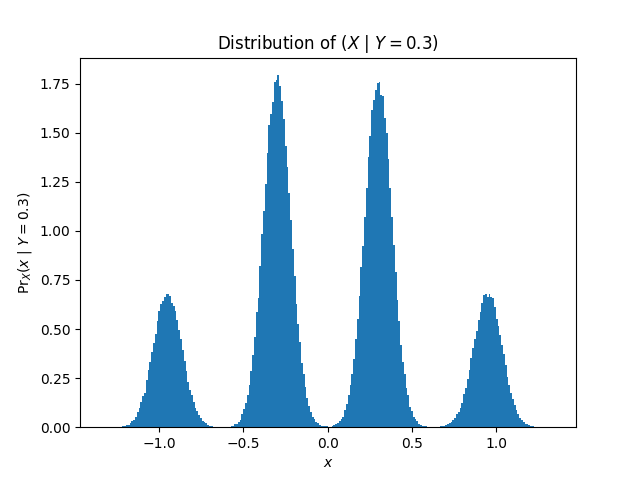
\includegraphics[width=0.6\textwidth]{
./distribution_of_x_given_y_is_nought_point_three}
\end{figure}

\end{enumerate}

\begin{examquestion}{2019}{6}{7}

\begin{enumerate}[label=(\alph*)]

\item Let $X_1, \dots, x_n$ be independent binary random variables,
$\mathbb{P}(X_i = 1) = \theta$, $\mathbb{P}(X_i = 0) = 1 - \theta$ for some
unknown parameter $\theta$. Using $\mathcal{U}[0, 1]$ as the prior
distribution for $\theta$, find the posterior distribution.

This is a standard result: the posterior distribution for $(\theta | X)$ is:
\[
\beta\left( 1 + \sum^n_{i=1}X_i, 1 + n - \sum^n_{i=1}X_i \right)
\]

We can find the posterior distribution using Bayes rule:

\[
\begin{split}
\text{Pr}(\theta \ | \ X)
&= \frac{\text{Pr}(\theta)\text{Pr}(X_1, \dots, X_n \ | \ \theta)}{\text{Pr}
(X_1, \dots, X_n)} \\
&= \kappa \cdot 1 \cdot \theta^{\sum^n_{i=1}X_i}(1 - \theta)^{n -
\sum^n_{i=1}X_i} \\
&= \kappa' \frac{n + 1}{n - \sum^n_{i=1}X_i} \theta^{\sum^n_{i=1}X_i}(1 - \theta)^{n -
\sum^n_{i=1}X_i}\\
\end{split}
\]

The distribution excluding $\kappa'$ is the probability density function for
a $\beta$ distribution with parameters $\left( 1 + \sum^n_{i=1}X_i, 1 + n -
\sum^n_{i=1}X_i \right)$.

Since both the whole distribution integrates to 1 over the range $\theta \in
[0, 1]$ and \\ $\frac{n + 1}{n - \sum^n_{i=1}X_i} \theta^{\sum^n_{i=1}X_i}(1 - \theta)^{n -
\sum^n_{i=1}X_i}$ integrates to 1 over the range $[0, 1]$, we can conclude
that $\kappa' = 1$ and therefore the posterior distribution is $\beta\left(
1 + \sum^n_{i=1}X_i, 1 + n - \sum^n_{i=1}X_i \right)$.

\item I have collected a dataset of images, and employed an Amazon
Mechanical Turk worker to label them. the labels are binary, nice
or nasty. To assess how accurate the worker is, I first picked 30
validation images at random, found the true label myself and compared to the
worker's label. The worker was correct on 25 and incorrect on 5.

Let $\theta$ be the probability that the worker labels an image incorrectly.
Using $\beta(0.1, 0.5)$ as the prior distribution for $\theta$, find the
posterior.

Let $1_{i}$ be the indicator variable for whether the worker labelled the
$i^\text{th}$ image correctly.

We can find the posterior distribution using Bayes rule:

\[
\begin{split}
\text{Pr}(\theta \ | \ 1_1, \dots, 1_{30})
&= \frac{\text{Pr}(\theta)\text{Pr}(1_1, \dots, 1_{30} \ | \ \theta)}{\text{Pr}(1_1, \dots, 1_{30})} \\
&= \kappa \theta^{0.1 - 1}(1 - \theta)^{0.5 -
1}\cdot\theta^{5}(1 - \theta)^{25} \\
&= \kappa \theta^{5.1 - 1}(1 - \theta)
^{25.5 - 1} \\
&= \kappa' \begin{pmatrix} 29.6 \\ 4.1 \\ \end{pmatrix} \theta^{5.1 - 1}(1 -
\theta)
^{25.5 - 1}
\end{split}
\]

The equation excluding $\kappa'$ is the probability density function for a
beta distribution $\beta\left( 5.1, 25.5 \right)$.

Since both the posterior probability and the $\beta$ component integrate to
1 over the range $\theta \in [0, 1]$; we can conclude that $\kappa' = 1$.
Therefore the posterior probability distribution is
equal to the probability density function for $\beta\left(5.1, 25.5 \right)$
and therefore the posterior probability has a beta distribution
parameters $(5.1, 25.5)$.

\item I next ask the worker to label a new test image, and they tell me the
image is nice. Let $z \in \{\text{nice}, \text{nasty}\}$ be the true
label and let the prior distribution for $z$ be $\text{Pr}(\text{nice})=0.1$,
$\text{Pr}(\text{nasty})=0.9$.

For both $z = \text{nice}$ and $z=\text{nasty}$, find:

\[
\mathbb{P}(\text{worker says nice} \ | \ z, \theta)
\]

Hence find the posterior distribution of $(z, \theta)$. Your answer may be
left as an un-normalised density function.

\begin{gather*}
    \mathbb{P}(\text{worker says nice} \ | \ \text{nice}, \theta) = 1 -
    \theta\\
    \mathbb{P}(\text{worker says nice} \ | \ \text{nasty}, \theta) = \theta\\
    \mathbb{P}(\text{worker says nice} \ | \ z, \theta) =
1_{z=\text{nice}}\left(1 - \theta\right) + 1_{z=\text{nasty}}\theta\\
\end{gather*}

We can find the posterior distribution of $(z, \theta)$ using Bayes rule:

\[
\begin{split}
\text{Pr}(z, \theta \ | \ \text{worker says nice}, 1_i, \dots, 1_{30})
&= \frac{\text{Pr}(z, \theta)\text{Pr}(\text{worker says nice}, 1_i, \dots, 1_{30} \ | \ z,
\theta)}{\text{Pr}(\text{worker says nice}, 1_i, \dots, 1_{30})} \\
&= \kappa \left(0.1\cdot 1_{z=\text{nice}}(1 - \theta) + 0.9\cdot
1_{z=\text{nasty}}\theta\right)\theta^{5.1 - 1}(1 - \theta)^{25.5 - 1} \\
\end{split}
\]

\item Find the posterior distribution of $z$:

We can find the posterior distribution for $z$ by integrating the posterior
distribution for $(z, \theta)$ with respect to $\theta$ between $0$ and $1$.

Let $\Pr(\theta, \alpha, \beta)$ be the pdf for the beta distribution with
parameters $(\alpha, \beta)$ evaluated at $\theta$.

\[
\begin{split}
& \text{Pr}(z \ | \ \text{worker says nice}, 1_1, \dots, 1_{30}) \\
=& \int^{1}_{0} \text{Pr}(z, \theta \ | \ \text{worker says nice}, 1_i,
\dots, 1_{30}) \text{d}\theta \\
=& \int^{1}_{0} \kappa \left(0.1\cdot 1_{z=\text{nice}}(1 - \theta) + 0.9\cdot
1_{z=\text{nasty}}\theta\right)\theta^{5.1 - 1}(1 -
\theta)^{25.5 - 1} \text{d}\theta \\
=& \int^{1}_{0} \kappa \left(0.1\cdot 1_{z=\text{nice}}\theta^{5.1 - 1}(1 -
\theta)^{26.5 - 1} + 0.9\cdot 1_{z=\text{nasty}}\theta^{6.1 - 1}(1 -\theta)
^{25.5 - 1}\right)\text{d}\theta \\
=& \int^{1}_{0} 0.1\kappa\begin{pmatrix}
30.6 \\ 4.1 \\ \end{pmatrix}^{-1} 1_{z=\text{nice}}\Pr(\theta, 5.1, 26.5) +
0.9\kappa \begin{pmatrix}
30.6 \\ 5.1 \\ \end{pmatrix}^{-1}1_{z=\text{nasty}}\Pr(\theta, 6.1, 25.5)
\text{d}\theta \\
=& 0.1\kappa\begin{pmatrix} 30.6 \\ 4.1 \\ \end{pmatrix}^{-1}
1_{z=\text{nice}}\int^{1}_{0}\Pr(\theta, 5.1, 26.5)\text{d}\theta + 0.9\kappa\begin{pmatrix}
30.6 \\ 5.1 \\ \end{pmatrix}^{-1}1_{z=\text{nasty}}\int^{1}_{0}\Pr(\theta, 6.1,
25.5)\text{d}\theta \\
\end{split}
\]

Since the integral of any beta distribution between 0 and 1 is 1, both the
integrals evaluate to 1. We substitute this in and then absorb some more terms
into $\kappa$. This gives the posterior probability:
\[
0.1\kappa\begin{pmatrix} 30.6 \\ 4.1 \\ \end{pmatrix}^{-1}
1_{z=\text{nice}} + 0.9\kappa\begin{pmatrix}
30.6 \\ 5.1 \\ \end{pmatrix}^{-1}1_{z=\text{nasty}} \\
\]

Since these probabilities must sum to 1, we can conclude that:
\[
\kappa = \frac{\begin{pmatrix} 30.6 \\ 5.1
 \\ \end{pmatrix} \cdot \begin{pmatrix} 30.6 \\ 4.1 \\ \end{pmatrix}}{0.1\begin{pmatrix} 30.6 \\ 5.1 \\ \end{pmatrix} +
0.9\begin{pmatrix} 30.6 \\ 4.1 \\ \end{pmatrix}}
\]

Therefore the posterior probability for $z$ is given by:

\[
\Pr(z \ | \ \text{data}) = 0.1\frac{\begin{pmatrix} 30.6 \\ 5.1
 \\ \end{pmatrix} }{0.1\begin{pmatrix} 30.6 \\ 5.1 \\ \end{pmatrix} +
0.9\begin{pmatrix} 30.6 \\ 4.1 \\ \end{pmatrix}}
1_{z=\text{nice}} + 0.9\frac{ \begin{pmatrix} 30.6 \\ 4.1 \\ \end{pmatrix}}{0.1\begin{pmatrix} 30.6 \\ 5.1 \\ \end{pmatrix} +
0.9\begin{pmatrix} 30.6 \\ 4.1 \\ \end{pmatrix}}1_{z=\text{nasty}}
\]

This equates to a probability of $35.7\%$ that the image is nice and
$64.3\%$ that the image is nasty. This passes the sanity check -- the worker
has shown that it is often correct and therefore the worker saying an image
is nice would mean the posterior probability of that image being nice should
be larger than the prior probability. Additionally, if the robot had been
more correct, the posterior probability for nice worked out using this method
would have been higher -- and if it had been less correct it would be lower.

\item My colleague has more grant money and she can employ 3 workers to rate
each image. On a test set of 30 images, she found that they all agreed on 15
images, worker 1 was the odd one out on 8 of the images, worker 2 was the
odd one out on 4, and worker 3 was the odd one out on 3.

Let $\theta_i$ be the probability that worker $i$ labels an image
incorrectly. Find the posterior distribution of $(\theta_1, \theta_2,
\theta_3)$. Your answer may be left as an un-normalised density function.

Let data be the described observations.

We can work out the posterior probability using Bayes' rule:

\[
\Pr(\theta_1, \theta_2, \theta_3 \ | \ \text{data})
= \frac{\Pr(\theta_1, \theta_2, \theta_3)\Pr(\text{data} \ | \ \theta_1, \theta_2, \theta_3)}{\Pr
(\text{data})}
\]

The probability of observing the data we have seen is equal to the
product of the probabilities of the observations. So if worker 1 and 2
guessed the same but 3 disagreed the probability of that observation would be
$\theta_1\theta_2(1 - \theta_3) + (1 - \theta_1)(1 - \theta_2)\theta_3$.
Therefore the total probability of observing all the data given $\theta_1,
\theta_2, \theta_3$ is:

\[
\begin{split}
\Pr(\text{data} \ | \ \theta_1, \theta_2, \theta_3) =&
(\theta_1\theta_2\theta_3 + (1 - \theta_1)(1 - \theta_2)(1 - \theta_3))
^{15}\times \\
& ((1 - \theta_1)\theta_2\theta_3 + \theta_1(1 - \theta_2)(1 - \theta_3))^8
\times\\
& (\theta_1(1 - \theta_2)\theta_3 + (1 - \theta_1)\theta_2(1 - \theta_3))^4
\times\\
&(\theta_1\theta_2(1 - \theta_3) + (1 - \theta_1)(1 - \theta_2)\theta_3)^3
\end{split}
\]

Denote the above probability $p(\theta_1, \theta_2, \theta_3)$

Therefore, using Bayes rule, the posterior probability is equal to:

\[
\begin{split}
\Pr(\theta_1, \theta_2, \theta_3 \ | \ \text{data})
&= \frac{\Pr(\theta_1, \theta_2, \theta_3)\Pr(\text{data} \ | \ \theta_1,
\theta_2, \theta_3)}{\Pr(\text{data})} \\
&= \kappa \theta_1^{-0.9}(1 - \theta_1)^{0.5}\theta_2^{-0.9}(1 - \theta_2)
^{0.5}\theta_3^{-0.9}(1 - \theta_3)^{0.5}p(\theta_1, \theta_2, \theta_3)\\
\end{split}
\]


\end{enumerate}

\end{examquestion}

\end{document}
